Afhankelijk van de versie van VirtualBox kan je via de de knop New of via de menubalk Machine en dan New een nieuwe virtuele machine aanmaken. Het eerste scherm waarmee je geconfronteerd wordt is \ref{VB_New_VM}.
\begin{figure}[H]
	\centering
	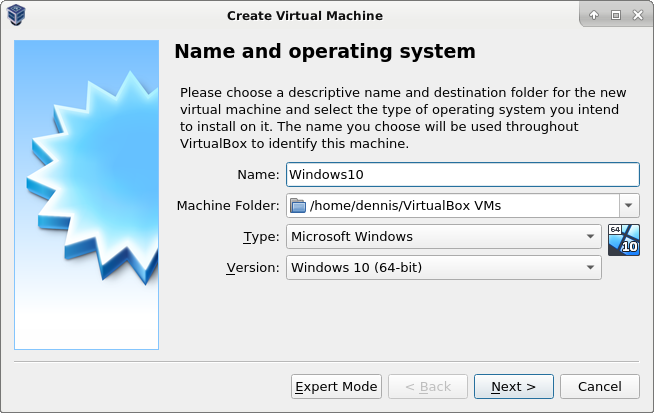
\includegraphics{virtualbox_vm_new.png}
	\caption{VirtualBox New VM}
	\label{VB_New_VM}
\end{figure}
Op het scherm wordt je gevraagd om de machine een naam te geven en er wordt gevraagd wat voor virtuele machine je wil aan maken. Op basis van de keuzes die je maakt bij Type en Version worden er later bepaalde standaard waarden gekozen, die je zelf natuurlijk nog kunt wijzigen. Type is het besturingssysteem en Version is de versie van het besturingssysteem dat je later wil gaan installeren.

Als je je keuzes gemaakt hebt mag je op Next klikken. Daarna zal het scherm verschijnen dat je de mogelijkheid geeft om de hoeveelheid RAM te kiezen die er aan de machine moet worden toegewezen (zie figuur \ref{VB_New_VM_RAM}). Over het algemeen zijn de default waarden goed, mocht je voor een opdracht andere waarden nodig hebben dan kan je ze natuurlijk wijzigen. Het voordeel van virtuele machines is dat je later makkelijk deze settings ook nog kan wijzigen, dus zelfs als je hier geen juiste waarde hebt gekozen, is dat later nog aan te passen. Bij de selectie van de hoeveelheid geheugen is het verstandig om niet meer RAM aan een VM toe te wijzen dan er in je machine zit min de hoeveelheid RAM die nodig is voor de op dat moment gebruikte hoeveelheid RAM. Dit om te voorkomen dat je systeem trager wordt doordat de VM alles gebruikt.

\begin{figure}[H]
	\centering
	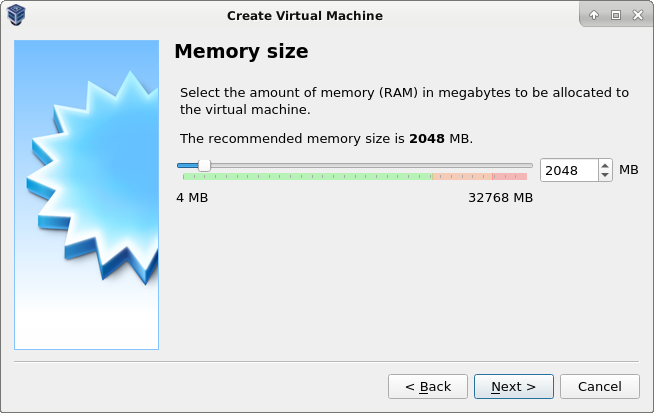
\includegraphics{virtualbox_vm_new_ram.png}
	\caption{VirtualBox New VM}
	\label{VB_New_VM_RAM}
\end{figure}

Na de keuze voor de hoeveelheid RAM komt de keuze voor de harddisk aanbod. Je kan kiezen uit geen harddisk (figuur \ref{VB_New_VM_HD}), het aanmaken van een nieuwe harddisk of het gebruiken van een bestaand disk-image. Dit is geen echte harddisk. De harddisk van een virtual machine is een bestand dat op de systeemharddisk wordt geschreven, een zogenaamde disk image. Je machine gebruikt dus een bestand als virtuele harddisk. Voor een nieuwe machine maken wij een nieuwe harddisk aan.

\begin{figure}[H]
	\centering
	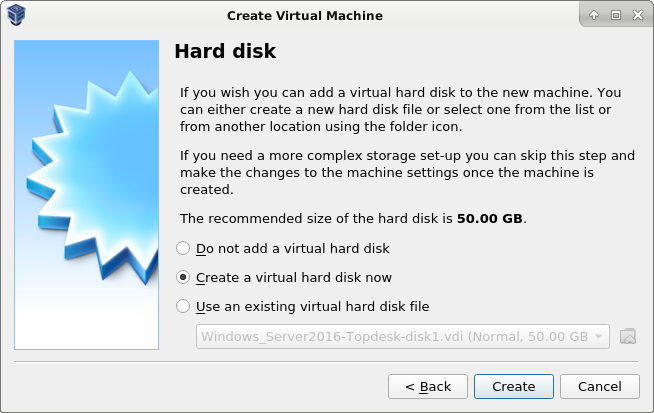
\includegraphics{virtualbox_vm_new_harddisk.png}
	\caption{VirtualBox New VM}
	\label{VB_New_VM_HD}
\end{figure}

Na op Next geklikt te hebben krijg je in \ref{VB_New_VM_HD_Type} de keuze voor het type disk image dat VirtualBox voor je moet aanmaken. Het standaard formaat van VirtualBox is VDI\index{VDI}\index{VirtalBox Disk Image}.

\begin{figure}[H]
	\centering
	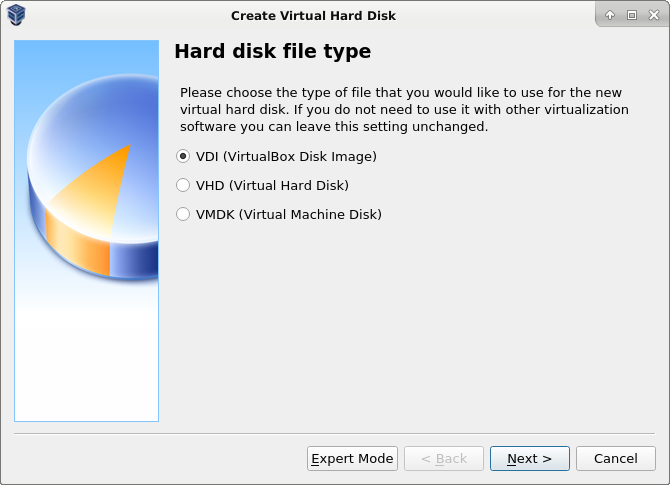
\includegraphics{virtualbox_vm_new_harddisk_type.png}
	\caption{VirtualBox New VM}
	\label{VB_New_VM_HD_Type}
\end{figure}

Omdat een VM volledig draait vanuit een bestand op de hardeschijf is er geen noodzaak om meteen alle ruimte in beslag te nemen. De virtuele disk kan dynamisch groeien met het gebruik van de virtuele machine. Een dynamisch groeiende disk is iets trager, maar neemt uiteindelijk minder ruimte in. Deze afweging moet je maken bij je keuze in het scherm dat je ziet in \ref{VB_New_VM_HD_Size}.

\begin{figure}[H]
	\centering
	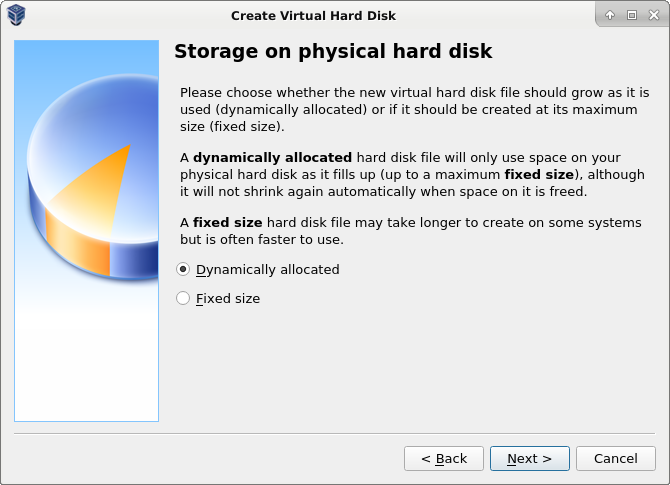
\includegraphics{virtualbox_vm_new_harddisk_size.png}
	\caption{VirtualBox New VM}
	\label{VB_New_VM_HD_Size}
\end{figure}

Tenslotte moet je nog bepalen waar het harddiskbestand en de overige gegevens over je VM worden opgeslagen (zie figuur \ref{VB_New_HD_Location}, ook hier geldt dat de default waarde meestal wel klopt en je kan hier de maximale ruimte voor de virtuele harddisk opgeven. Ook hier is weer een default waarde gegeven. Bepaal zelf of dit ook het formaat is van de harddisk die je wilt hebben. Let er daarbij vooral op dat je niet meer opgeeft dan je vrije diskruimte hebt.

\begin{figure}[H]
	\centering
	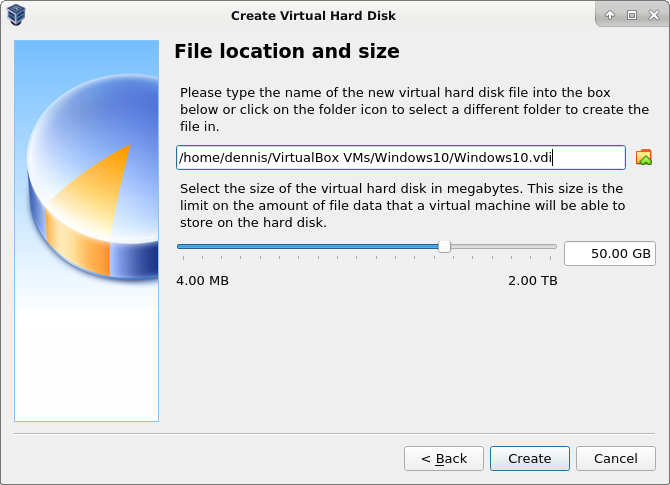
\includegraphics{virtualbox_vm_new_harddisk_location.png}
	\caption{VirtualBox New VM}
	\label{VB_New_VM_HD_Location}
\end{figure}

Klik op Create om de virtuele machine te maken.
